\documentclass{beamer}
\usepackage[T2A]{fontenc}
\usepackage[utf8]{inputenc}
\usepackage[english,russian]{babel}
\usepackage{graphicx}

\usepackage{beamerthemesplit} % new
\usetheme{Goettingen}
\usecolortheme{seahorse}
% \usefonttheme{structureitalicserif}
\hypersetup{unicode=true}

% \usepackage[unicode]{hyperref}

\begin{document}
\title{Direlog}
\author{Андрей Тропин}

\institute{
  К06-682 \\
  НИЯУ МИФИ \\
  Москва \\
  \texttt{andrewtropin@gmail.com}
}

\date{\today}

\frame{\titlepage}

% \frame{\frametitle{Содержание}\tableofcontents}


\section{Цели}

\frame{
  \frametitle{Цели}
  \begin{block}{Уменьшение времени реагирования на инциденты}
    Ускорение диагностики проблем runtime-поиска(верхнего метапоиска)
  \end{block}
}

\section{Постановка задач}
\subsection{Краткое описание архитектуры}
\frame{
  \frametitle{Краткое описание архитектуры поиска}
    \begin{column}{.94\textwidth}
      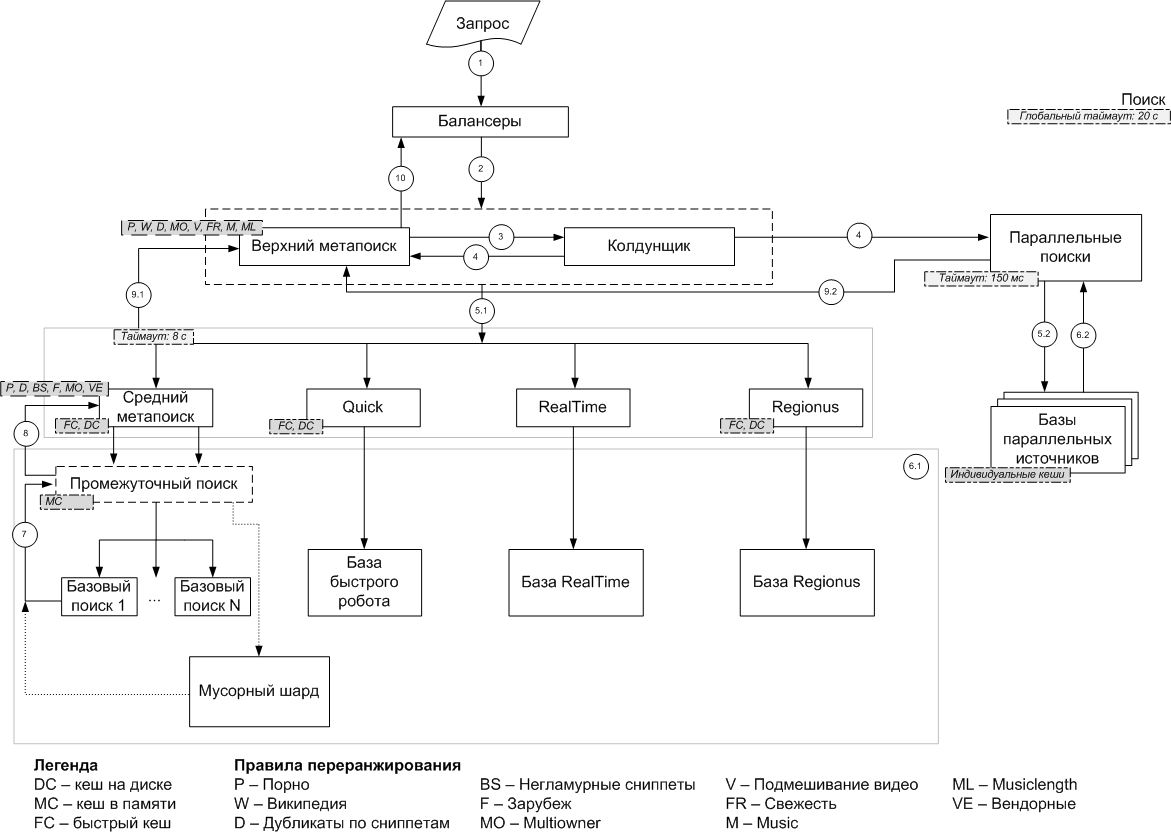
\includegraphics[width=\textwidth]{./search.png}
    \end{column}
}

\subsection{Проблемы}
\frame{
  \frametitle{Проблемы}
  \begin{block}{error\_log}
    Файл содержащий ошибки верхнего метапоиска, как со стороны вёрстки(V8), так и со стороны репорта(perl-ового кода)
  \end{block}
  \begin{itemize}
    \item Большое количество шума
    \item Отсутствие классификации ошибок по важности
    \item Невозможность быстрого определения источника ошибки
    \item Сложность оценки масштаба инцидента
  \end{itemize}
}

\subsection{Задачи}
\frame{
  \frametitle{Задачи}
  Реализовать следующие функциональные возможности:
  \begin{itemize}
    \item Первоначальная подготовка лога
    \item Хранение и версионирование паттернов
    \item Получение сниппета(ов) по паттерну
    \item Подсчёт статистики
    \item Выделение ``неизвестных`` ранее ошибок
    \item Добавление нового паттерна к существующим
  \end{itemize}
}

\section{Результаты}
\subsection{Итог работы}
\frame{
  \frametitle{Итог работы}
  \begin{itemize}
    \item Разработано приложение
    \item Благодаря статистическим отчётам и технологии skynet появилась возможность значительно ускорить рефакторинг существующей системы вывода ошибок
    \begin{itemize}
      \item Устранено 4 часто встречающихся типа ошибок, бесполезных во время инцидента
      \item Уменьшен объем лога генерируемого в единицу времени в 2 раза. С 32Мб до 15Мб за два часа.
      \item Менеджерами команд запланированы субботники
    \end{itemize}

  \end{itemize}
}
\subsection{Пример использования}
\frame{
  \frametitle{Пример использования}
    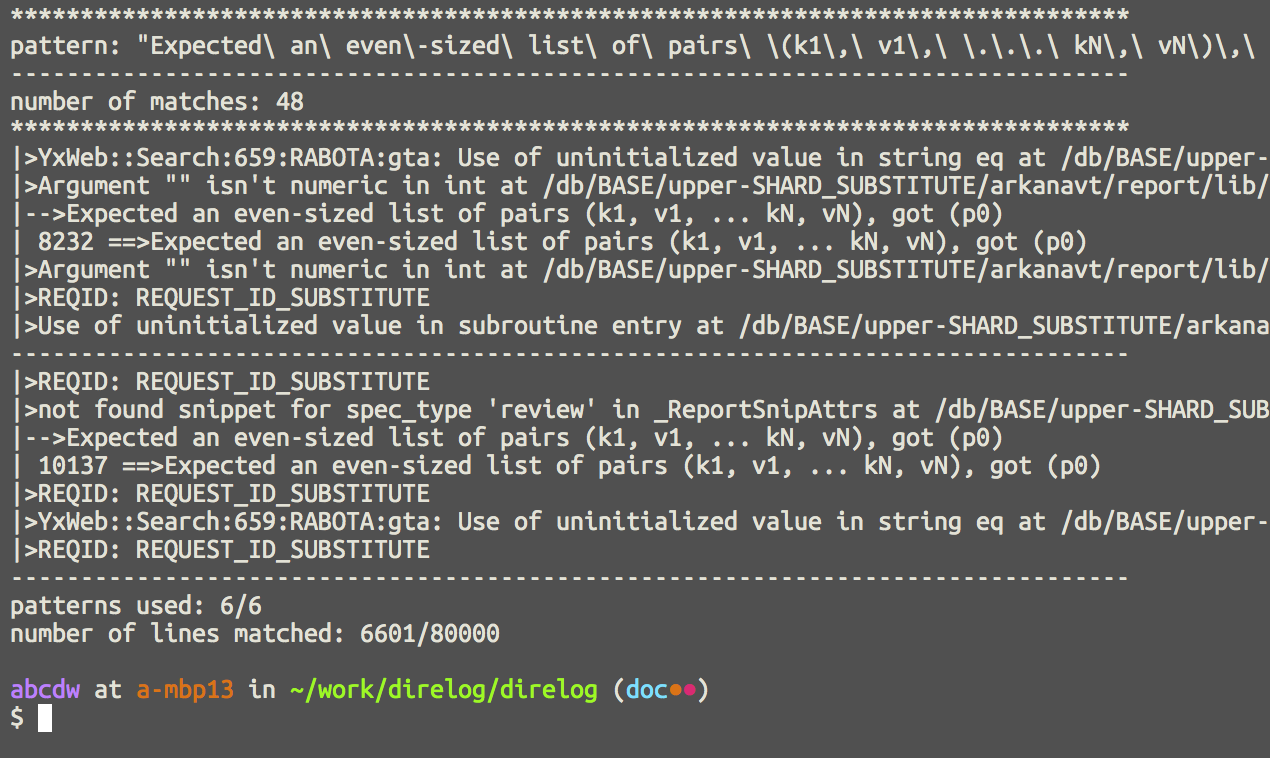
\includegraphics[width=\textwidth]{./direlog.png}
  % \begin{itemize}
    % \item
  % \end{itemize}
}

\subsection{Дальнейшие действия}
\frame{
  \frametitle{Дальнейшие действия}
  \begin{itemize}
    \item Планируется внедрение приложения на продуктовый кластер. И оценка повышения эффективности реагирования на инциденты, связанные с проблемами верхнего метапоиска.
    \item Планируется доработка приложения с целью запуска на MapReduce-кластере.
  \end{itemize}
}

\section{Конец}
\frame{
  \frametitle{Конец }
  \begin{center}
    Спасибо за внимание. Вопросы?
  \end{center}
}

\end{document}

